\chapter{Convolution}

Convolution is an operation which takes two functions and produces a third.
It takes one of the two input functions, and modifies one by mirroring and translating.
The resulting function is then the overlap between one of these functions as a function of the translation.
Visually, this can be seen below in Figure~\ref{fig:ConvolutionExample}.

+1 line

\begin{figure}[ht]
	\caption[Convolution of box signal with itself]{The convolution of the box signal 
	$f(t)=g(t)=\left( 0^\oiOpOp{-\infty,-0.5} \oplus 1^\oiClCl{-0.5,0.5} \oplus 0^\oiOpOp{0.5,\infty} \right)$ with itself.
	\emph{(from wikipedia; need to create new versions)}
	\label{fig:ConvolutionExample}}
	\centering
	\includegraphics[scale=0.5]{diagrams/conv1}
	\includegraphics[scale=0.5]{diagrams/conv2}
	\includegraphics[scale=0.5]{diagrams/conv3}
\end{figure}

Formally this, equates to the following definition for convolution over continuous domains:
\begin{definition}
	The \textbf{convolution} $*$, of two functions $F$ and $G$ is defined as:
	\begin{equation}
		(F*G)(t) = \int_{-\infty}^\infty F(\tau) \;G(t - \tau) \; d\tau
	\end{equation}
\end{definition}
and in the case of discrete linear convolution, summation would replace integration.
In this equation, $t$ represents the translation of $G$ as well as the input for $(F*G)$
while $\tau$ is internal to the integral and varies over the real line.


\begin{figure}[ht]
	\caption[Gaussian Blurring]{512x512px ``Lena''(a) with a 1px (b) and 5px (c) Gaussian blur applied. 
	Gaussian blurring is accomplished by convolving an image with a Gaussian kernel and is commonly used
	in image processing to reduce noise prior to edge detection.
	\label{fig:LenaBlur}}
	\centering
	\begin{subfigure}[b]{0.3\textwidth}
                \includegraphics[scale=0.25]{diagrams/Lenna}
                \caption{Original Image}
       \end{subfigure}
       \begin{subfigure}[b]{0.3\textwidth}
                \includegraphics[scale=0.25]{diagrams/Lenna-blur1}
                \caption{1px Gaussian blur}
       \end{subfigure}
       \begin{subfigure}[b]{0.3\textwidth}
                \includegraphics[scale=0.25]{diagrams/Lenna-blur5}
                \caption{5px Gaussian blur}
       \end{subfigure}
\end{figure}


Convolution has applications in many areas of mathematics and engineering.
One very common use in image processing is in blurring.
\emph{Gaussian blurring} is the result of a 2-dimensional convolution of an image with the Gaussian distribution function:
\begin{equation}
	\label{eqn:2dGaussian}
	G(x,y) = \frac{1}{2 \pi \sigma^2} \; \text{exp} \left( - \frac{x^2 + y^2}{2\sigma^2} \right)
\end{equation}
Blurring an image in this way reduces noise and greatly increases the efficacy of subsequent edge detection.
In statistics, a (simple) \emph{moving average} can be represented as a convolution by a rectangular pulse while more
generally, weighted moving averages can be made by convolving with other functions.





%%%%%%%%%%%%%%%%%%%%%%%%%%%%%%%%%%%%%%%%%
%
% CONVOLUTION OF PIECEWISE
%
%%%%%%%%%%%%%%%%%%%%%%%%%%%%%%%%%%%%%%%%%
\section{Convolution of Piecewise Functions}


CAS such as Maple and Mathematica are quite adept at solving integrals.
Convolution of elementary functions generally poses no problem.
When convolving two piecewise continuous functions, many possible intervals arise and the conditionals that arise
can quickly overwhelm them unaided. \todo{cite, rewrite?}


We are interested in \emph{Symbolic Linear Convolution} (of piecewise continuous functions).
The typical approach is to first consider for convolution of ``one piece'' functions 
\cite{evans1994algorithms, west1993symbolic}.
By ``one-piece'' functions we mean functions which are restricted to a single interval and zero everywhere else.
We will consider two functions, $F$ and $G$ defined as:


\begin{equation}
	\label{eqn:fOnePiece}
	F(x)=f^{[a_f,b_f)}(x) = 
		\begin{cases}
			f(x) & a_f \leq x < b_f \\
			0 & \text{otherwise}
		\end{cases}
\end{equation}
\begin{equation}
	\label{eqn:gOnePiece}
	G(x)=g^{[a_g,b_g)}(x) = 
		\begin{cases}
			g(x) & a_g \leq x < b_g \\
			0 & \text{otherwise}
		\end{cases}
\end{equation}
for which we would like to compute the convolution $(F*G)$.
To reduce the total number of cases generated, it is generally also assumed that $b_f - a_f \leq b_g - a_g$.
Assuming that $F$ is non-zero over a shorter interval is not that strong an assumption as convolution is commutative;
if it is not the case we can rearrange $F*G$ to $G*F$.
To see this, simply apply the substitute $\tau' = t-\tau$ in equation (7.1):
\begin{align}
	\label{eqn:ConvCommutative}
	(F*G)(t) 
		&= \int_{-\infty}^\infty F(\tau) G(t-\tau) \;d \tau 
		\notag\\&= \int_{\infty}^{-\infty} F(t-\tau')G(\tau')\; (-1) d\tau' 
		\notag\\&= \int_{-\infty}^\infty G(\tau') F(t-\tau') \; d\tau'
		\notag\\&= (G*F)(t)
\end{align}


Thus we can assume that our static function is also the function with the shorter interval.
Since $F$ and $G$ are zero outside of their respective intervals, we do not need to integrate over the entire real line. 
$F$ is our static function, so $[a_f, b_f)$ would be sufficient.
For a tight boundary, we have the following:
\begin{align}
	\label{eqn:ConvNaiveOnePiece}
	(F*G)(t) 
	&= \int_{-\infty}^\infty F(\tau)\; G(t-\tau) \; d\tau \notag \\
	&= \int_{a_f}^{b_f} f(\tau) \; G(t-\tau) \; d\tau \notag \\
	&= 	\begin{cases}
			\int_{a_f}^{t-a_g} f(\tau) \; g(t-\tau) \; d\tau 	& (a_f+a_g) \leq t < (b_f+a_g) \\
			\int_{a_f}^{b_f} f(\tau) \; g(t-\tau) \; d\tau		& (b_f+a_g) \leq t < (a_f+b_g) \\
			\int_{t-b_g}^{b_f} f(\tau) \; g(t-\tau) \; d\tau	& (a_f+b_g) \leq t < (b_f+b_g) \\
			0										& \text{otherwise}
		\end{cases}
\end{align}


\begin{figure}[ht]
	\caption[Convolution of ``one-piece'' functions]{Convolution of length 1 and 2 rectangular pulses. 
	Given the functions $F=1^{[-2,2)}$ and $G=1^{[-1,1)}$, there are three non-zero regions in $(F*G)$.
	\label{fig:OnePiece}}
	\centering
	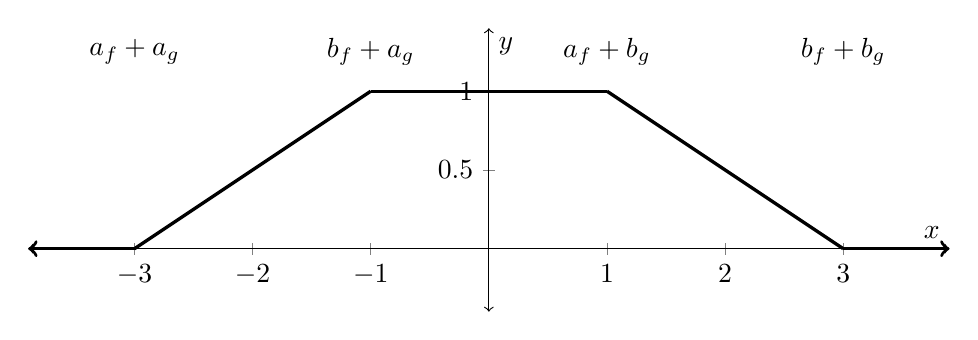
\begin{tikzpicture}
		\begin{axis}[
			x=1.5cm,
			y=2cm,
			xstep=1,
			ystep=1,
			xmin=-3.9,xmax=3.9,
			ymin=-0.4,ymax=1.4,
			axis x line=middle,
			axis y line=middle,
			axis line style=<->,
			xlabel={$x$},
			ylabel={$y$},
	        ]
		\addplot[no marks,black,very thick,<-] expression[domain=-3.9:-3,samples=100]{0};
		\addplot[no marks,black,very thick,-] expression[domain=-1:1,samples=100]{1};
		\addplot[no marks,black,very thick,-] expression[domain=-3:-1,samples=100]{(.5*x)+1.5};
		\addplot[no marks,black,very thick,-] expression[domain=1:3,samples=100]{1.5-(.5*x)};
		\addplot[no marks,black,very thick,->] expression[domain=3:3.9,samples=100]{0};
		\node(afag) at (axis cs:-3,1.25) {$a_f+a_g$};
		\node(bfag) at (axis cs:-1,1.25) {$b_f+a_g$};
		\node(afbg) at (axis cs:1,1.25) {$a_f+b_g$};
		\node(bfbg) at (axis cs:3,1.25) {$b_f+b_g$};
	        \end{axis}
		%\draw[thick,<->] (-4,0) -- (4,0);
		%\draw[thick,<->] (0,-.5) -- (0,1.5);
		
	\end{tikzpicture}
\end{figure}


These regions can be visualized as above in Figure~\ref{fig:OnePiece} where two rectangular pulses are convolved. 
If both functions had equal length non-zero intervals (i.e. $b_f-a_f = b_g-a_g$), then the central plateau would be empty
(as in Figure~\ref{fig:ConvolutionExample}).
Another formulation presented by C\^{i}rnu \cite{cirnu2012calculation} and Cavicchi \cite{cavicchi2002simplified} is to use:
\begin{equation}
	\label{eqn:ConvCirnu}
	(F*G)(t)=
	\begin{cases}
		\int_{\max(a_f, \; t-b_g)}^{\min(b_f, t-a_g)} f(\tau)\cdot g(t-\tau)\; d\tau & (a_f+a_g) \leq t < (b_f+b_g) \\
		0 & \text{otherwise}
	\end{cases}
\end{equation}
Although this may appear to reduce the number of cases, expanding the $\min$ and $\max$ will cause just as many 
cases to return.


To extend this to piecewise continuous function, 
we simply treat each piecewise function as the sum of ``one-piece'' functions.
Given functions, $F= \sum_i f_i^{P_i}$ and $G= \sum_j g_j^{Q_j}$ 
where $\{P_i\}$, $\{Q_j\}$ are each sets of disjoint intervals, and $f_i^{P_i}$, $g_j^{Q_j}$ are all ``one-piece'' functions.
The convolution of $F*G$ is the sum of pairwise convolution:

\begin{align}
	\label{eqn:ConvPiecewise}
	\left(\left(\sum_i f_i^{P_i}\right) * \left(\sum_j g_j^{Q_j}\right)\right) (t)
	&= \int_{-\infty}^\infty \left(\sum_i f_i^{P_i}\right)(\tau)\cdot \left(\sum_j g_j^{Q_j}\right)(t-\tau) \;d\tau
	\notag\\&= \sum_i \sum_j \int_{-\infty}^\infty f_i^{P_i}(\tau) \cdot g_j^{Q_j}(t-\tau) \;d\tau 
	\notag\\&= \sum_i \sum_j \left(f_i^{P_i} * g_j^{P_j}\right)
\end{align}


This is the typical approach to convolution of piece-wise functions originally presented by West and McClellan 
\cite{west1993symbolic}.
When the boundaries between regions is symbolic, then we may not be able to determine which interval is longer.
Concerns with intervals where one boundary point is at infinity have also been raised \cite{evans1994algorithms}.








%%%%%%%%%%%%%%%%%%%%%%%%%%%%%%%%%%%%%%%%%
%
% HYBRID CONVOLUTION
%
%%%%%%%%%%%%%%%%%%%%%%%%%%%%%%%%%%%%%%%%%
\section{Hybrid Function Convolution}

With hybrid functions we do not have to worry about the relative length of $f$ and $g$ intervals.

Instead for hybrid functions $F = f^{[a_f, b_f)}$ and $G = g^{[a_f, b_f)}$:

\begin{align}
	(F \;*\; G) (t) = 
		\mathcal{R}_+ &\left( \; \left( 
			\int_{a_f}^{x-a_g} f(\tau) \; g(t-\tau) \; d\tau \right)^{[\![a_f+a_g,\; b_f+a_g)\!)} 
				\right. \notag \\ &\oplus \left( 
			\int_{a_f}^{b_f} f(\tau) \; g(t-\tau) \; d\tau \right)^{[\![b_f+a_g,\; a_f+b_g)\!)} 
				\notag \\ &\oplus \left. \left( 
			\int_{x-b_g}^{b_f} f(\tau) \; g(t-\tau) \; d\tau \right)^{[\![a_f+b_g,\; b_f+b_g)\!)} 
				\; \right)(t)
\end{align}

When $b_f - a_f \leq b_g - a_g$ then the intervals will be disjoint and the expression is identical to 2.61

Otherwise, the interval $[\![b_f +a_g, \; a_f + b_g)\!)$ will have a negative orientation.

For $(a_f+b_g) \leq t < (b_f+a_g)$ then $t$ will be in all three regions and we have


%%%%%%%%%%%%%%%%%%%%%%%%%%%%%%%%%%%%%%%%%
%
% INFINITE INTERVALS
%
%%%%%%%%%%%%%%%%%%%%%%%%%%%%%%%%%%%%%%%%%
\section{Infinite Intervals}\label{sec:ConvInfty}



%%%%%%%%%%%%%%%%%%%%%%%%%%%%%%%%%%%%%%%%%
%
% EXAMPLE
%
%%%%%%%%%%%%%%%%%%%%%%%%%%%%%%%%%%%%%%%%%
\section{Example}

\newpage